\documentclass{article}
\usepackage[utf8]{inputenc}
\usepackage{dirtytalk}
\usepackage{caratula}
\usepackage{amssymb}
\usepackage{amsmath}
\usepackage{geometry}
\usepackage{fixltx2e}
\usepackage{wrapfig}
\usepackage{cite}
\usepackage{grffile}
\graphicspath{{../experimentos}{.}}

\geometry{
 a4paper,
 total={210mm,297mm},
 left=30mm,
 right=30mm,
 top=30mm,
 bottom=30mm,
 }
 
\begin{document}

\fecha{03 / 06 / 2015}
\materia{Métodos Numéricos}
\titulo{Recuperatorio del Trabajo Práctico 1}
\subtitulo{Si nos organizamos recuperamos rápido...}
\grupo{     
\\
}

\integrante{Abdala, Leila}{950/12}{abdalaleila@gmail.com}
\integrante{Albertini, Alejandro}{924/12}{ale.dc@hotmail.com}
\integrante{Bayardo, Julián}{850/13}{julian@bayardo.com.ar}
\integrante{Niesz, Ignacio}{}{ignacio.niesz@gmail.com}

\maketitle

\tableofcontents

\newpage

Este informe fue realizado en simultaneo con el tp. El codigo del tp no funciona como se espera, es decir, no pasa los tests de la catedra. Las situaciones aqui planteadas estan consideradas en el caso ideal. 
Entregamos de todos modos para presentar una idea del trabajo realizado hasta este momento y del que vamos a realizar cuando solucionemos los problemas de implementacion. No es nuestra intencion que se corrija este tp como si 
estuviese completo y para evitarles perdidas de tiempo informamos este problema. Sin embargo, nos interesa en gran medida recibir una opinion sobre el avance y la direcccion del trabajo. Lamentamos no poder
 completar el trabajo en el lapso estipulado, pero nos comprometemos a entregar un trabajo de calidad en la siguiente fecha. Sin mas, les presentamos el informe.

\section{Introducci\'on}

En este informe se detalla el dise\~no e implementaci\'on de algoritmos que modelan los metodos de Eliminaci\'on Gaussiana y factorizaci\'on LU,
para resoluci\'on de sistemas de ecuaciones lineales. Tambien se presentan algoritmos para la aplicaci\'on de la formula de Sherman-Morrison y
una estructura para el almacenamiento de matrices banda, con el fin de mejorar la complejidad espacial y la temporal. Luego de realizamos una %extremadamente 
breve experimentaci\'on para analizar la calidad de las soluciones, performance de los algoritmos, realismo del modelado, etc.

Esto se realiza al resolver un problema practico mendiante el modelado y discretizaci\'on del mismo. Este problema consiste en, dado un parabrisas 
P que esta siendo atacado por sanguijuelas mutantes, a las que llamaremos $S_i$, averiguar la temperatura del punto critico que se
halla en el centro de P. P cuenta con un sistema de refrigeracion que mantiene el borde a temperatura constante
$-100^o$C. Cada sanguijela $S_i$ cuenta con una pocision $(x_i, y_i)$, un radio $r_i$ y una temperatura $t_i$. Si un punto del
parabrisas, $P_{k,j}$, 
pertenece al area afectada por algun $r_i$ y no pertenece al borde de P, la temperatura de dicho punto es $t_i$, donde por area afectada nos referimos a la circunsferencia de 
radio $r_i $ y centro $(x_i, y_i)$. Si pertenece a mas de un radio, es decir
$P_{k,j} \in {r'_i}, i\in (1..l) $, entonces su temperatura sera 
$t_{k,j}=max_{i\in (1..l)}(r'_i) $. Si el punto $P_{k,j}$ no pertenece a ninguno de los anteriores,
su temperatura esta determinada por la siguiente formula:


\begin{equation}\label{eq:calor}
\frac{\partial^2T(x,y)}{\partial x^{2}}+\frac{\partial^2 T(x,y)}{\partial y^{2}} = 0.
\end{equation}

Ademas, si el punto critico supera los $235^o $C, se desea saber si eliminando tan solo una sanguijuela, y cual es dicha sanguijuela,
se puede lograr que la 
temperatura se redusca por debajo de este margen, pues de lo contrario el parabrisas se rompera.

Como P tiene una superficie continua y dado que es imposible representar valores continuos en una PC,
debemos discretizar nuestro sistema. Por lo tanto vamos a modelar la superficie de P de tal forma que P sea representado por una matriz de
temperaturas. Es decir, solo consideraremos los puntos h-distantes para el modelado, donde h es un parametro del problema. 
%Por simplicidad, se asume que el ancho y el largo, a y b respectivamente, son multiplos de h.
Solo seran afectados por una sanguijuela $S_i$ los puntos h-distantes que esten incluidos en el radio de $S_i$. Si el radio de una sanguijuela $S_i$ no 
afecta ningun punto de la discretizacion, esta no se tendra en cuenta en la modelizacion del problema. 

Una vez discritezado el problema de esta manera, podemos$^2$ estimar la ecuacion (1) de la siguiente forma:
\begin{equation}
t_{ij} \ =\ \frac{ t_{i-1,j} + t_{i+1,j} + t_{i,j-1} + t_{i,j+1}}{4}.\label{eq:calordd}
\end{equation}

\footnotetext[2]{ Explicaci\'on al respecto en el apendice A}

%Por lo tanto, obtenemos la siguiente funcion de temperatura global (lo completare si me viene en gana)

A partir de este modelo, despejando las ecuaciones de calor, obtenemos un sistema de ecuaciones lineales.
Para la resolucion del sistema resultante, vamos a aplicar dos metodos. Estos seran Eliminaci\'on Gaussiana y factorizaci\'on LU.

En el caso de que debamos decidir que sanguijuela eliminar, aplicaremos en primera instancia la tecnica de Backtraking. Luego aplicaremos
la formula de Sherman-Morrison, para optimizar. 

Detallando los m\'etodos utilizados, notamos que el m\'etodo de Eliminacion Gaussiana consta de dos pasos: en primer
lugar, transforma el sistema original a uno equivalente donde la matriz es triangular
superior, con costo $O(n^3)$ donde n es el n\'umero de inc\'ognitas. Luego procede a resolver dicho
sistema, con costo $O(n^2)$. Por otro lado, el m\'etodo de descomposici\'on LU descompone el sistema original
$Ax = b$ en un sistema del tipo $LUx = b$, donde $L$ es una matriz triangular inferior y $U$ es una matriz
triangular superior, con costo $O(n^3)$. Luego resuelve los sistemas $Ly = b$ y
$Ux = y$ para obtener el valor de soluci\'on $x$, con costo $O(n^2)$ en cada caso. 
En t\'erminos asint\'eticos ambos m\'etodos tienen una $complejidad O(n^3)$, sin embargo, la factorizaci\'on LU presenta 
una ventaja por sobre EG. Si el sistema se debe resolver para un b diferente, no hace falta realizar nuevamente la factorizaci\'on,
sino que simplemente basta con resolver los dos sistemas triangulares usando las mismas matrices L y
U lo que resulta en un costo cuadratico, en lugar del costo cubico asociado a la Eliminaci\'on Gaussiana. \\\\

Notese ademas que para las matrices de este problema se puede$^3$ aplicar Eliminacion Gaussiana sin pivotear, o lo que es lo mismo, existe Factorizaci\'on LU
\footnotetext[3]{Para una demostracion de esta propiedad consulte a su docente amigo de Metodos Numericos.}

\section{Desarrollo}

\subsection{Sobre la implementación}
En principio, y con la intención de entender el problema en profundidad, planteamos un ejemplo que resolvimos manualmente. A partir de este ejemplo
notamos un patrón en el comportamiento del sistema. Por lo tanto recrearemos a continuación dicho ejemplo, para dar una noción clara de nuestra 
evolución en la comprensión de este problema particular.

Asumamos que recibimos un archivo de entrada con los siguientes parámetros:\\

3 \ \ \ \   3  \ \ \ \ 1 \ \ \ \ 1\\
2.5  \ \ \ \ 2.5 \ \ \ \ 1  \ \ \ \ 500

entonces el problema modelado es de la pinta$^6$:\footnotetext[6]{Aclaramos
que la circunferencia negra representa una sanguijuela mutante y el cuadrado celeste, al parabrisas.}

\begin{figure}[]
    
\includegraphics[width=0.3\textwidth]{ejP01}
    \caption{Imagen ilustrativa del parabrisas}
\end{figure}

Luego lo representaremos como muestra el gráfico a continuación, donde cada intersección de las lineas representa una variable del modelo, de la cual
debemos averiguar su temperatura.

\begin{figure}[]
    
\includegraphics[width=0.3\textwidth]{ejP02}
    \caption{Representación visual del modelo discretizado}
\end{figure}

Notar que, si bien C, D y H pertenecen al radio de una sanguijuela, al formar parte del borde están condicionados por el sistema de refrigeración,
por lo cual su temperatura es $-100$ en lugar de $500$.

Planteando la ecuación de temperatura para cada variable y despejando, obtenemos el siguiente sistema de ecuaciones $Ax=B$:
\begin{equation}
 a\ =\ -100
\end{equation}
\begin{equation}
 b\ =\ -100
\end{equation}
\begin{equation}
 c\ =\ -100
\end{equation}
\begin{equation}
 d\ =\ -100
\end{equation}
\begin{equation}
 e\ =\ -100
\end{equation}
\begin{equation}
 f - \frac{b}{4} - \frac{e}{4} - \frac{g}{4} - \frac{j}{4}\ =\ 0
\end{equation}
\begin{equation}
 g\ =\ 500
\end{equation}
\begin{equation}
 h\ =\ -100
\end{equation}
\begin{equation}
 i\ =\ -100
\end{equation}
\begin{equation}
 j- \frac{f}{4} - \frac{i}{4} - \frac{k}{4} - \frac{n}{4}\ =\ 0
\end{equation}
\begin{equation}
 k- \frac{g}{4} - \frac{j}{4} - \frac{l}{4} - \frac{o}{4}\ =\ 0
\end{equation}
\begin{equation}
 l\ =\ -100
\end{equation}
\begin{equation}
 m\ =\ -100
\end{equation}
\begin{equation}
 n\ =\ -100
\end{equation}
\begin{equation}
 o\ =\ -100
\end{equation}
\begin{equation}
 p\ =\ -100
\end{equation}

 del cual la matriz asociada $A$ es la siguiente:
 
%Matriz del sistema
\begin{center}
   \begin{tabular}{| c | c | c | c | c | c | c | c | c |c | c |c | c |c | c | c | c | c | c | c | c |c | c |c | c |c | c |c | c |}
     \hline
       & a  & b & c & d & e & f & g & h & i & j & k & l & m & n & o & p  \\ \hline
   (3) & 1  & 0 & 0 & 0 & 0 & 0 & 0 & 0 & 0 & 0 & 0 & 0 & 0 & 0 & 0 & 0 \\ \hline
   (4) & 0  & 1 & 0 & 0 & 0 & 0 & 0 & 0 & 0 & 0 & 0 & 0 & 0 & 0 & 0 & 0 \\ \hline
   (5) & 0  & 0 & 1 & 0 & 0 & 0 & 0 & 0 & 0 & 0 & 0 & 0 & 0 & 0 & 0 & 0 \\ \hline
   (6) & 0  & 0 & 0 & 1 & 0 & 0 & 0 & 0 & 0 & 0 & 0 & 0 & 0 & 0 & 0 & 0 \\ \hline
   (7) & 0  & 0 & 0 & 0 & 1 & 0 & 0 & 0 & 0 & 0 & 0 & 0 & 0 & 0 & 0 & 0 \\ \hline
   (8) & 0  & $-\frac{1}{4} $ & 0 & 0 & $-\frac{1}{4} $ & 1 & $-\frac{1}{4} $ & 0 & 0 & $-\frac{1}{4} $& 0 & 0 & 0 & 0 & 0 & 0 \\ \hline
   (9) & 0  & 0 & 0 & 0 & 0 & 0 & 1 & 0 & 0 & 0 & 0 & 0 & 0 & 0 & 0 & 0 \\ \hline
   (10) & 0  & 0 & 0 & 0 & 0 & 0 & 0 & 1 & 0 & 0 & 0 & 0 & 0 & 0 & 0 & 0 \\ \hline
   (11) & 0  & 0 & 0 & 0 & 0 & 0 & 0 & 0 & 1 & 0 & 0 & 0 & 0 & 0 & 0 & 0 \\ \hline
   (12) & 0  & 0 & 0 & 0 & 0 & $-\frac{1}{4} $ & 0 & 0 & $-\frac{1}{4} $ & 1 & $-\frac{1}{4} $ & 0 & 0 & $-\frac{1}{4} $ & 0 & 0 \\ \hline
   (13) & 0  & 0 & 0 & 0 & 0 & 0 & $-\frac{1}{4} $ & 0 & 0 & $-\frac{1}{4} $ & 1 & $-\frac{1}{4} $ & 0 & 0 & $-\frac{1}{4} $ & 0 \\ \hline
   (14) & 0  & 0 & 0 & 0 & 0 & 0 & 0 & 0 & 0 & 0 & 0 & 1 & 0 & 0 & 0 & 0 \\ \hline
   (15) & 0  & 0 & 0 & 0 & 0 & 0 & 0 & 0 & 0 & 0 & 0 & 0 & 1 & 0 & 0 & 0 \\ \hline
   (16) & 0  & 0 & 0 & 0 & 0 & 0 & 0 & 0 & 0 & 0 & 0 & 0 & 0 & 1 & 0 & 0 \\ \hline
   (17) & 0  & 0 & 0 & 0 & 0 & 0 & 0 & 0 & 0 & 0 & 0 & 0 & 0 & 0 & 1 & 0 \\ \hline
   (18) & 0  & 0 & 0 & 0 & 0 & 0 & 0 & 0 & 0 & 0 & 0 & 0 & 0 & 0 & 0 & 1 \\ \hline
   \end{tabular}
\end{center}

siendo la ecuación (3) la resultante de despejar la ecuación de temperatura para la variable $a$, (4) para la variable $b$ y así sucesivamente.
Ordenándolo de esta manera, la matriz asociada $A$ es una matriz banda de ancho y altura n, donde n es la cantidad de columnas 
de la matriz de temperaturas. Esto lo deducimos observando la figura 2 y la matriz A,
ya que notamos que para averiguar el valor de la variable $v_{i}$ son necesarios$^7$ los valores de las variables $v_{i-n}$, $v_{i-1}$, 
$v_{i+1}$, $v_{i+n}$, donde n hace referencia a la cantidad de columnas.
\footnotetext[7]{Siempre y cuando $v_{i}$ no pertenezca a un borde o este cubierta por una sanguijuela.}
Notar que en las ecuaciones, o lo que es lo mismo, matriz asociada al sistema no se hicieron remplazos previos. Con esto nos referimos a no reemplazar
 en las ecuaciones de calor automáticamente los valores conocidos, como los del borde o los afectados por sanguijuelas. Un ejemplo de esto se daría 
 al usar las ecuaciones (4), (7) y (9) para reemplazar los valores en la ecuación (8). Tomamos esta decisión porque consideramos que esos reemplazos son parte
 de la resolución total del sistema, por lo que deberían verse reflejados en la medición de tiempos. Sin embargo, si hiciéramos los reemplazos 
 en la generación de la matriz asociada al sistema, no podríamos medirlos con confiabilidad pues tendríamos la lectura de datos como outlier. También debemos tener en cuenta el caso de que, por algún motivo, se deba cambiar el valor de la temperatura de los bordes. Dise\~nado de este modo, tenemos mayor escalabilidad^8. \footnotetext[8]{Buscando siempre seguir las buenas practicas de programación}

Dejaremos el ejemplo hasta aquí, pues la resolución del sistema no aporta información útil. Sin embargo, una vez que hallamos esta estructura 
procedimos a realizar la carga de datos de modo que la matriz asociada a nuestro sistema fuese una matriz banda-n. Ahora explicaremos el desarrollo del código.
%\footnotetext[8]{Por dato del enunciado, en ese momento sabiamos que debimos obtener una matriz banda a partir del sistema, si bien no sabiamos como organizar los datos para obtenerla.}

El lenguaje empleado para la implementación es C++. Si bien la elección del lenguaje podría considerarse arbitraria, se debió principalmente a la gran
cantidad de herramientas y librerías provistas por este lenguaje, a diferencia de la otra opción dada por la cátedra. 


Luego de implementada Eliminación Gaussiana y Factorizaci\'on LU, procedimos a crear la interfaz del problema en si, es decir la entrada y salida de datos, la generación
del sistema, etc. Establecimos como criterio usar el promedio de las temperaturas, de todos los puntos que estén
en el interior en la circunferencia de radio h con centro en el punto crítico,
para la estimación de la temperatura del mismo. En particular, si el punto critico es un punto de la discretizaci\'on, entonces es el único punto en el interior de la circunferencia.

Para finalizar la implementación, programamos el Algoritmo Simple para calcular cual sanguijuela eliminar,
y algoritmo mejorado con la fórmula de Sherman-Morrison. 


%%%%%Yo no me hago cargo de lo que dice entre los %%%
La fórmula de Sherman-Morrison nos permite conseguir un sistema equivalente al de $(A+B)^{-1}x=b$ si podemos encontrar dos vectores $u$ y $v$
tales que $uv^t=B$.

Sherman-Morrison nos proponen la siguiente Formula:

$x = (A + uv^{t})^{-1} b = A^{-1}b -  \dfrac{v^{t}A^{-1}b}{1+v^{t}A^{-1}u} A^{-1}u$

Pero sabemos que:

$A^{-1}b = y \iff Ay = b 
A^{-1}u = z \iff Az = u $

Suponiendo que ya resolvimos el sistema A antes de la modificacion, tenemos su descomposicion, $ LU=A $. Por lo que basta resolver: $\\\
Ly_{2} = y $ y $ Lz_{2}=z$

Luego, $ Uy=y_{2} $ y $ Uz=z_{2}$
Una vez calculados $ y $ y $ z $ estamos en condiciones de resolver la expresion. Notemos que

$ \dfrac{v^{t}A^{-1}b}{1+v^{t}A^{-1}u} $ es un escalar.

Finalmente $ x = y +  \dfrac{v^{t}y}{1+v^{t}z} z$


En cuanto a $ uv^{t} $ recordemos que vamos a usar sherman-morrison para sistemas que cambiar una sola fila i, por lo que nos basta con
conseguir que $ uv^{t} $ sea una matriz que modifique apropiadamente dicha fila. Por lo tanto tomamos a $u$ como el i-esimo vector de la base canonica,
y a $v$ como la modificacacion que nesesitamos para tranformar la fila i.








%sola componente/coordenada. Por lo que podemos suponer que la modificacion sera: $ A + \alpha E_{ij} $ donde 
%$ \alpha = \beta - A_{ij} $ con $\beta $ el nuevo valor para la posicion y $ E_{ij} $ la matriz con todos $ 0 $ excepto un $ 1 $ en la posicion $i,j $.
%Ademas sabemos que $ E_{ij} = e_{i} e^{t}_{j} $ donde $ e_{i} $ es el vector como fila con todos ceros excepto un uno en la posicion $ i $ y $ e^{t}_{j} $ es el vector como columna con todos ceros excepto un uno en la posicion $ j $.
%Finalmente $A + uv^{t} =A +\alpha e_{i} e^{t}_{j}$.
%Es decir si cambiamos la posicion $ i, j $ por el valor $ \beta $ tomamos $ uv^{t} = \alpha e_{i} e^{t}_{j}$.

%%%%%%Leila.

\subsubsection{Pseudocódigo}

\subsection{Sobre la experimentación}

Para medir los tiempos de resolución, utilizamos la función gettimeof day, que permite medir con
facilidad el lapso de tiempo entre dos momentos de la ejecución del programa. Decidimos medir
únicamente los tiempos que estuvieran estrictamente relacionados a la resolución del sistema,
dejando afuera, por ejemplo, el tiempo empleado para escribir las soluciones en archivos de salida. La
idea de fondo que nos llevó a medir de esta manera fue la de intentar que las magnitudes de los tiempos
empleados por los métodos de triangulación de Gauss y LU no se vieran afectadas por tiempos mucho
mayores que distorsionaran la distancia relativa entre ellas.

Una vez finalizada la etapa de implementación y testeo de los algoritmos, procedimos a realizar una
serie de experimentos que nos permitieran evaluar el comportamiento de los mismos. Además de
analizar como se modifican los resultados a medida que se modifica el parámetro de discretización
h, definimos algoritmos para comparar el desempeño, en términos de la estimación de temperaturas.
Por comodidad, a la hora de diseñar los experimentos, definimos todos los parabrisas con forma cuadrada.

Siguiendo la consigna del TP, planteamos tres casos diferentes para analizar como varia la temperatura 
en el punto critico al variar la discretización. Estos casos fueron generados de manera pseudo aleatoria. Es decir, si bien las posiciones de las sanguijuelas se establecieron usando una distribución uniforme y la temperatura usando una distribución normal~\cite{proba}, restringimos los rangos de ambos parámetros para lograr la instancia deseada.


%Finalmente, corrimos los experimentos utilizando MatLab. Elegimos este programa principalmente
%porque permite obtener de una manera simple los gr ́aficos que queriamos mostrar. A su vez, nuestras
%decisiones de implementacion de “main.cpp” y “armaInFile.py” nos permitieron automatizar en gran
%medida el proceso de experimentacion, por lo cual no nos demando excesivo tiempo implementar esta
%etapa del desarrollo (si lo demando el tener que pensar que experimentos realizar y como mostrar
%los resultados). Los experimentos de MatLab tienen como salida los graficos que presentamos en la
%siguiente seccion.

\section{Experimentación}

Presentaremos en esta sección la experimentación y discusión juntas, para cada experimento. Primero daremos una breve descripción de la instancia experimental, seguido de lo que esperamos observar, es decir, nuestra hipótesis. A continuación mostraremos los 
resultados obtenidos y nuestro análisis respecto a por qué obtuvimos dichos resultados.

\subsection{Metodología en la generación de instancias}

Para la creación de instancias de prueba, por una cuestión de practicidad, y para evitar sesgar los experimentos, decidimos utilizar instancias generadas aleatoriamente utilizando numpy. Todo el código de generación de datos, así como de corrida de tests, y las instancias utilizadas para la experimentación, se encuentran en la carpeta experimentos. En términos de las distribuciones utilizadas, en cada uno de los experimentos explicaremos las particularidades de la elección de distribución, pero aquí presentamos una tabla mostrando la distribución utilizada para la generación de los parámetros de las sanguijuelas:

\begin{center}
\begin{tabular}{l | l | l | l | l | l | l}
Experimento & Instancia & \#Sanguijuelas & X & Y & Radio & Temperatura\\ \hline
$1$ & $1$ & $50$ & $\mathcal{U}(45, 55)$ & $\mathcal{U}(45, 55)$ & $|\mathcal{N}(0.5, 10)|$ & $\mathcal{E}(1/100)$\\ \hline
$1$ & $2$ & $50$ & $\mathcal{U}(0, 100)$ & $\mathcal{U}(0, 100)$ & $|\mathcal{N}(2, 100)|$ & $\mathcal{E}(1/100)$\\ \hline
$1$ & $3$ & $50$ & $\mathcal{U}(0, 100)$ & $\mathcal{U}(0, 100)$ & $|\mathcal{N}(0.1, 10)|$ & $\mathcal{E}(1/300)$\\ \hline
$2$ & $1$ & $50$ & $\mathcal{U}(0, 100)$ & $\mathcal{U}(0, 100)$ & $\mathcal{U}(0, 10)$ & $\mathcal{E}(1/300)$\\ \hline
$3$ & $1$ & $31$ & Explicado & Explicado & Explicado & $\mathcal{E}(1/300)$\\ \hline
\end{tabular}
\end{center}

Todas las instancias son de $100x100$. En el caso del experimento 3 tomamos $h = 1$ para simplificar la generación de instancias, mientras que en los otros casos utilizamos

$$h \in \{0.5, 0.8, 1.0, 1.25, 2.0, 2.5, 4.0, 5.0, 6.25, 10.0, 12.5\}$$

Explicaremos más en profundidad estas decisiones en las subsecciones correspondientes. La elección de los valores de $h$ fue una tarea complicada: la restricción de $h | a \wedge h | b$ restringe ampliamente el conjunto de valores; fuera de eso, utilizar valores de granularidad demasiado pequeños aumenta demasiado el costo computacional, como veremos más adelante. Encontramos que intentar correr las instancias con un $h < 0.5$ elevaba demasiado el costo temporal de resolver el problema, por lo que utilizamos este valor como punto de comienzo.

\subsection{Experimento 1: temperatura en función de la granularidad}

Para este experimento, nos planteamos como objetivo estudiar la relación entre la matriz de temperaturas final, la granularidad, y la distribución de las sanguijuelas. Desde el punto de vista algorítmico, notemos que la granularidad impacta en las sanguijuelas que terminan determinando la temperatura inicial de los puntos: si una sanguijuela es lo suficientemente chica y está ubicada de forma tal que su radio no llega a impactar en el punto de la discretización más cercano, no será considerada como parte de la matriz. Más aun, es importante advertir que las elecciones impuestas sobre el modelado generan condiciones extrañas: cuando dos sanguijuelas se superponen en un punto, se tomará el máximo de las temperaturas como la inicial para el punto. Es decir, existen instancias donde el aumento de granularidad (y por lo tanto la aparición de sanguijuelas de radio pequeño) efectivamente termina borrando sanguijuelas que antes existían, reemplazándolas por otras de mayor temperatura. Lo que buscamos remarcar con esto es que es difícil predecir el efecto que va a tener el cambio de granularidad sobre la matriz final de temperaturas cuando comienzan a haber más sanguijuelas, ya que la interacción de la discretización con las mismas se vuelve cada vez más complicada.

El primer experimento que ideamos consiste en crear una instancia donde todas las sanguijuelas estén muy cercanas al punto crítico, con radios lo suficientemente pequeños como para que el efecto de desaparición que mencionamos antes logre entrar en acción. Tras un largo proceso de prueba y error, determinamos que las distribuciones mencionadas anteriormente eran las que mejor modelaban la idea intuitiva que estábamos buscando probar. En particular, la elección de una distribución exponencial se debe a que buscamos que las sanguijuelas tengan valores relativamente pequeños para que borrarlas logre mostrarnos un cambio concreto en la temperatura del punto crítico. Para todos los casos del experimento 1 utilizamos el método de eliminación gaussiana para obtener las matrices de temperatura correspondientes.

Intuitivamente esperábamos que la temperatura en el punto crítico fuera aumentando a medida que achicásemos el $h$: suponíamos que aumentar la granularidad forzosamente iba a resultar en que la mayor temperatura de las sanguijuelas cercanas al centro tomase relevancia en el punto crítico e iba a hacer que la temperatura del mismo subiese, mientras que tener una menor granularidad debía hacer que cada vez más sanguijuelas se perdieran en la discretización y forzaría a que las sanguijuelas mejor posicionadas para los nuevos valores de $h$ dominen la temperatura en el punto crítico. De las instancias que corrimos, creemos que el gráfico \ref{fig:exp11} es ampliamente representativo.

\begin{figure}[b]
    \centering
    \includegraphics[width=0.685\textwidth]{experimento 1-1}
    \caption{Variación de la temperatura en función de la granularidad para la primera instancia}
    \label{fig:exp11}
    
    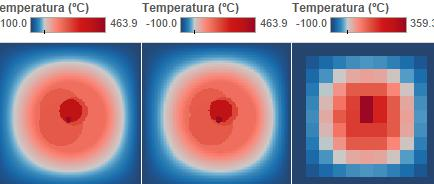
\includegraphics[width=0.685\textwidth]{Ejemplo Instancia 1}
    \caption{Mapa de calor para la instancia 1}
    \label{fig:exp11-vis}
\end{figure}

Es fácil observar que la temperatura del punto critico se estabiliza a medida que aumenta la granularidad, y tiende a ser más bien caótico a medida que aumentamos el valor de h, es decir, disminuimos la granularidad. A diferencia de lo que esperábamos, la temperatura con mayor granularidad no es la mayor de las obtenidas, encontramos que la granularidad de la discretización es más bien un parámetro de regulación para la precisión de la solución: cuanta mayor granularidad, más difícil es que las sanguijuelas que aparezcan cambien sustancialmente la temperatura del punto crítico, ya que un $h$ más pequeño implica que los radios de las sanguijuelas que quedan por descubrir son lo suficientemente chicos como para afectar pocos puntos, y la ecuación de calor parece "balancear" las temperaturas hacia los valores más frecuentes. A modo de ayudar a la comprensión del experimento y la instancia contemplada, creamos una visualización del mapa de temperaturas generado por esta instancia particular, variando los valores de $h$:

Observemos que a medida que disminuimos la granularidad, el borde con temperatura $-100$ºC comienza a tomar cada vez más relevancia dentro de la discretización, y colabora aun más que antes a reducir los valores de temperatura.

\pagebreak

Para la segunda instancia pensamos en crear sanguijuelas de un radio grande, en comparación con la primera instancia, alejadas del punto critico. En este caso esperábamos, en principio, que la temperatura se mantuviese constante a medida que aumentamos la granularidad, pues las sanguijuelas son lo suficientemente grandes para no desaparecer dentro de la discretización y más aun, esperamos una variación pequeña de temperatura en relación al aumento del $h$. Observemos que en este caso cambiamos completamente la forma de generar las instancias de test, quitando restricciones en tanto a los valores de las sanguijuelas: el hecho de tomar distribución uniforme para las posiciones nos asegura la existencia de sanguijuelas en una variedad de puntos de la discretización, mientras que el radio normal nos da acceso a un panorama más variado en términos de los radios.

\begin{figure}[b]
    \centering
    \includegraphics[width=0.685\textwidth]{experimento 1-2}
    \caption{Variación de la temperatura en función de la granularidad para la segunda instancia}
    \label{fig:exp12}
    
    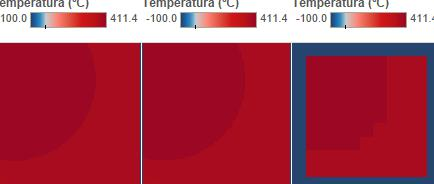
\includegraphics[width=0.685\textwidth]{Ejemplo Instancia 2}
    \caption{Mapa de calor para la instancia 2}
    \label{fig:exp12-vis}
\end{figure}

La justificación de porque la temperatura se estabiliza cercano a los $410$ºC es por qué hay una sanguijuela de aproximadamente $411$ºC y un radio muy grande, eso hace que abarque a muchos puntos de la discretización por más variación del h que haya. Con su radio, llega hasta el punto crítico y siempre le gana en temperatura a las sanguijuelas cercanas, ya que es la de mayor temperatura en esta instancia, y eso hace que le aumente la temperatura a los puntos de la discretización que no tienen sanguijuelas cercanas, como por ejemplo los puntos cercanos al centro del parabrisas pero que están del otro lado de la sanguijuela más caliente y no tienen ninguna sanguijuela a su alrededor. Al promediarse la temperatura en esos puntos, hace que la temperatura en el punto crítico sea cercana a los $410$ºC.

Observemos, en la figura \ref{fig:exp12}, que efectivamente la diferencia de temperatura entre el primer y el último h es baja, menor a $5$ºC, confirmando nuestra hipótesis sobre la variación de la temperatura a lo largo del aumento de granularidad. Una vez más encontramos que el algoritmo converge a una solución a partir de cierto $h$ y se mantiene estable, aunque la diferencia en este caso es que el $h$ viene antes que en la instancia 1. Una vez más, proveemos una visualización de la clase generada para la instancia 2 en el gráfico \ref{fig:exp12-vis}

\pagebreak

Como tercera instancia, nos planteamos ver qué sucede con las sanguijuelas más pequeñas al estar alejadas del centro. Para esto, generamos instancias con las distribuciones mencionadas anteriormente, pero observemos que en este caso tomamos la temperatura como una variable exponencial de esperanza $300$, es decir, tomamos valores de temperatura mucho más altos. Nuestro análisis de los casos anteriores nos induce a pensar que las sanguijuelas suficientemente peque\~nas no tendrán tanta relevancia en la temperatura del punto critico. Esto es porque, al afectar pocos puntos de la discretizaci\'on, la ecuación de calor compensa esos valores al alejarse de la posición de las sanguijuelas. 

\begin{figure}[b]
    \centering
    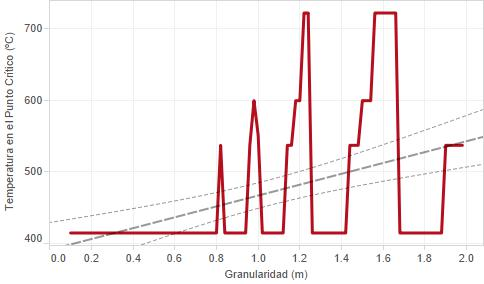
\includegraphics[width=0.685\textwidth]{experimento 1-3}
    \caption{Variación de la temperatura en función de la granularidad para la tercera instancia}
    \label{fig:exp13}
    
    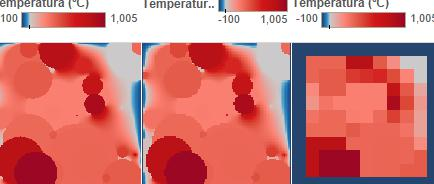
\includegraphics[width=0.685\textwidth]{Ejemplo Instancia 3}
    \caption{Mapa de calor para la instancia 3}
    \label{fig:exp13-vis}
\end{figure}

En el gráfico \ref{fig:exp13} podemos observar que la temperatura solo varia, para una granularidad muy baja, en el orden de los $20$ºC. Sin embargo, a diferencia de los casos anteriores, encontramos que la temperatura se estabiliza a valores cada vez mas bajos al aumentar la granularidad, que efectivamente es lo que hipotetizamos que sucedería. Para profundizar la comprensión, podemos ver en el gráfico \ref{fig:exp13-vis} los mapas de calor correspondientes a la tercera instancia.
\\
   Al tener un radio tan chico la mayoría de las sanguijuelas, por más alta que sea su temperatura, no va a afectar a gran cantidad de puntos. Por ejemplo tenemos la sanguijuela de temperatura máxima que es de $1000$ºC, sin embargo,  por más distinta que sea la discretización, la temperatura nunca supera los $270$ºC (para los valores de h probados), ya que al estar tan separada del centro y no tener un radio tan grande, no abarca muchos puntos de la discretización y la temperatura se va perdiendo a medida que nos vamos acercando al punto crítico.
\\
Nótese a medida que aumenta la granularidad la disipación de temperatura aumenta. En particular, nos concentramos en las sanguijuelas de mayor temperatura. Vemos que, en el mapa de mayor granularidad, parece que los altos valores de temperatura se limitan al área cubierta por las mismas, mientras que la temperatura desciende drásticamente al salir del radio. Se puede, sin embargo, observar áreas de calor entre dos sanguijuelas relativamente cercanas, donde la función de disipación debe disipar calor en dos direcciones contrarias. Observado esto, solo podemos concluir que las sanguijuelas de mayor temperatura están demasiado alejadas entre si, por lo que las altas temperaturas se pierden automáticamente en la ecuación.

Naturalmente, el algoritmo de factorización LU debería devolver exactamente las mismas matrices de temperatura (ya que resuelven el mismo problema). Comprobamos de cualquier forma en nuestra experimentación que esto funcionaba así como forma de testear la correctitud del código fuera de las instancias provistas por la cátedra.

\pagebreak

\subsection{Experimento 2: relación entre tiempo de cómputo y calidad de la solución}

Para este experimento, buscábamos complementar los conocimientos adquiridos en el experimento anterior: sabíamos que cuanta mayor granularidad teníamos, más precisa es nuestra solución, y teníamos claro que tomar valores de $h$ muy pequeños no nos permitía solucionar los problemas por la excesiva carga computacional. Ahora lo que faltaba entender mejor es cuál es la relación entre el costo computacional y la granularidad. Para esto, utilizamos la tercera instancia que habíamos creado en el experimento anterior y medimos los tiempos de ejecución del algoritmo, la metodología utilizada fue correr el programa $5$ veces por cada valor de $h$, y tomar el promedio de los tiempos reportados.

En el gráfico \ref{fig:exp21} podemos observar, en el primer casillero, la comparación entre los algoritmos, mientras que el segundo muestra la dimensión de la matriz del sistema a resolver (un punto $(h, d)$ en el gráfico se corresponde con una matriz final de $d \times ([\frac{a}{h}] + 1)$, tomaremos de aquí en adelante a $n$ como este $d$). Observemos que las filas de la matriz del sistema crecen a la razón de $f(h) = ([\frac{a}{h}] + 1)([\frac{b}{h}] + 1)$, que es una función decreciente, con límite a $+\infty$ cuando $h$ tiende a $0$. Es importante destacar que este gran crecimiento de la matriz impacta muy fuertemente sobre el costo computacional, ya que ambos algoritmos son $O(n^3)$ a pesar de las mejoras que alcanzamos explotando la estructura de banda de la matriz.

En concreto, tenemos que el costo de realizar eliminación gaussiana y resolver el sistema usando backward substitution es de $\frac{2n^3}{3} + \frac{3n^2}{2} + O(n)$ para sistemas que no precisan hacer pivoteo ~\cite{burden} (cabe destacar que esto no contempla las optimizaciones que realizamos para explotar la estructura de banda). Mientras tanto, realizar la factorización LU y resolver utilizando forward y backward substitution toma $\frac{2n^3}{3} + 2n^2 + O(n)$ ~\cite{LUComplexity}. Observemos que el costo de la factorización LU es mayor por un sumando de $\frac{n^2}{2}$, pero la explosión de complejidad que terminamos teniendo en las filas de la matriz hacen que este $n$ se dispare, generando la amplia diferencia que vemos en el gráfico \ref{fig:exp21}.

\begin{figure}[b]
    \centering
    \includegraphics[width=0.685\textwidth]{experimento 2-1}
    \caption{Comparación entre EG y LU}
    \label{fig:exp21}
\end{figure}



\pagebreak

\subsection{Experimento 3: comparación entre algoritmos para eliminación de sanguijuelas}

En este experimento nos enfocamos en analizar las diferencias entre los algoritmos de eliminación de sanguijuelas, a los que llamaremos eliminación simple y eliminación con Sherman-Morrison. Basados en los tests de correctitud, podemos afirmar que ambos algoritmos tienen el mismo comportamiento cualitativo. Es decir, ambos devuelven la misma solución. Por esto, el enfoque de este experimento es el análisis temporal de los experimentos. 

Antes de establecer hipótesis alguna, vamos a hacer un breve análisis del comportamiento esperado de cada algoritmo.

En primer lugar tenemos el algoritmo de eliminación simple. Este algoritmo se limita a, iterando sobre todas las sanguijuelas, eliminar una y recalcular la matriz de temperatura. Este comportamiento es independiente de los atributos de las sanguijuelas en si, sino que, a primera vista, es esperable que la complejidad solo dependa de la cantidad de sanguijuelas.

Luego tenemos eliminación con Sherman-Morrison. En este caso, si se vuelve relevante el radio de las sanguijuelas, ya que este algoritmo se evita recalcular toda la factorizaci\'on si la sanguijuela afecta solo un punto de la discretizaci\'on. 

Es por esto, que dise\~namos nuestro experimento de modo que se pueda apreciar la diferencia en el modo de cómputo. Este consiste en un tablero de $100 \times 100$ mts$^2$, en el cual fijaremos la cantidad de sanguijuelas y el tamaño de la discretizaci\'on. Para medir la performance de cada algoritmo, vamos a variar el radio de las sanguijuelas. Es decir, variaremos el porcentaje de sanguijuelas que solo afectan a un punto de la discretizaci\'on. Generamos instancias con $31$ sanguijuelas, incrementando el porcentaje de sanguijuelas unitarias que se encontraban en cada instancia con diferencias de aproximadamente $10\%$. Todas las instancias se caracterizan por tomar $h = 1$, y disponer de las sanguijuelas en forma de grilla, es decir, ocupando las posiciones en orden desde la esquina inferior derecha por filas, hasta lograr cubrir las posiciones necesarias. Además, posicionamos una sanguijuela de $1000$ºC en el punto crítico, para asegurarnos que los algoritmos corran al tener la misma por encima de $235$ºC. La forma de generar sanguijuelas unitarias es, entonces, a través de tomar radios menores a $0.8$ y mayores a $0.2$, mientras que en el caso dual podemos tomar sanguijuelas de radio mayor a $1.1$ y menor a $1.4$. Observemos que el incremento podemos determinarlo como "aproximadamente" de $10\%$ debido a que las sanguijuelas "unitarias" que se encuentren en el límite con las sanguijuelas no unitarias van a tener su posición influenciada por más de 1 sanguijuela, haciendo que no pueda aplicarse Sherman Morrison. De cualquier forma, esta limitación no generó ninguna complicación, ya que el cambio en el porcentaje es lo suficientemente bajo como para poder analizar los resultados de la misma forma. 

\begin{figure}[h]
    \centering
    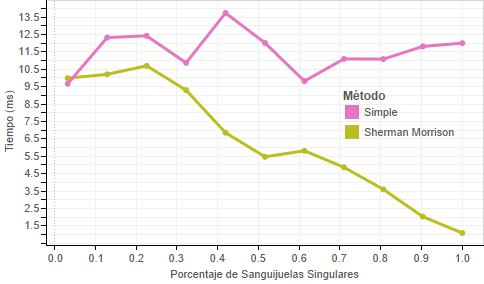
\includegraphics[width=0.685\textwidth]{experimento 3-1}
    \caption{Comparación entre SM y el método simple}
    \label{fig:exp31}
\end{figure}

Si miramos los tiempos de ejecución para Sherman-Morrison, podemos observar claramente que a medida que aunmenta el porcentaje de sanguijuelas unitarias, el tiempo de computo disminuye. Esto se debe a que cada vez que debe analizar una sanguijuela unitaria, puede aprovechar los resultados ya calculados, en lugar de recalcular la matriz entera, derivando en un menor costo computacional a medida que disminuye el radio de las sanguijuelas.

Por su parte, el algoritmo de elimacion simple mantiene un rango bajo de variacion en las mediciones. Esto sucede porque independientemente del rango de las sanguijuelas, siempre debe recalcular el total de los datos al eliminar una. 

Si comparamos la primer medicion, donde todas las sanguijuelas afectan mas de un punto de la discretizacion, podemos notar que eliminacion con Sherman-Morrison


\section{Conclusiones generales}

\bibliographystyle{unsrt}
\bibliography{citas}

\end{document}
